
Each of the once-through transition scenarios are compared on multiple 
criteria: the number of advanced reactors deployed, \hl{the energy profile?}, 
the mass of enriched 
uranium required, the amount of \gls{SWU} capacity required to enrich uranium,
and the mass of waste produced. A subset of these results are presented
in \cite{bachmann_enrichment_2021}, except the \glspl{LWR} were assumed to 
operate for 60 years if not closed before December 2020. 

\section{Scenario 1}
Scenario 1 models only the \glspl{LWR} deploying the United States with no 
perscribed energy demand. 

\begin{figure}
    \centering
    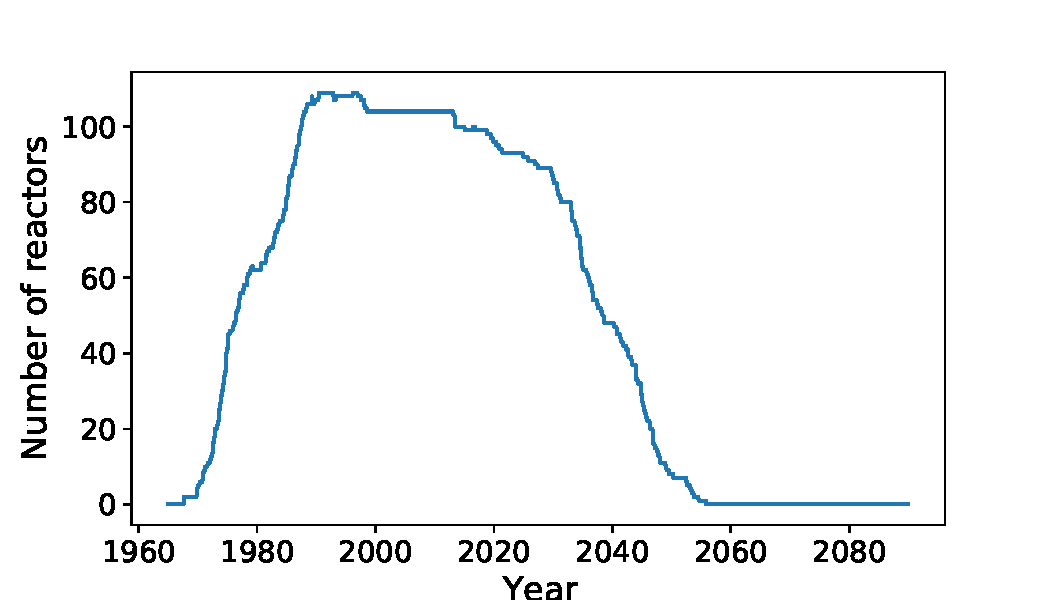
\includegraphics[scale=0.8]{s1_reactors.pdf}
    \caption{Number of LWRs deployed at each time step in Scenario 1.}
    \label{fig:reactor1}
\end{figure}

\begin{figure}
    \centering
    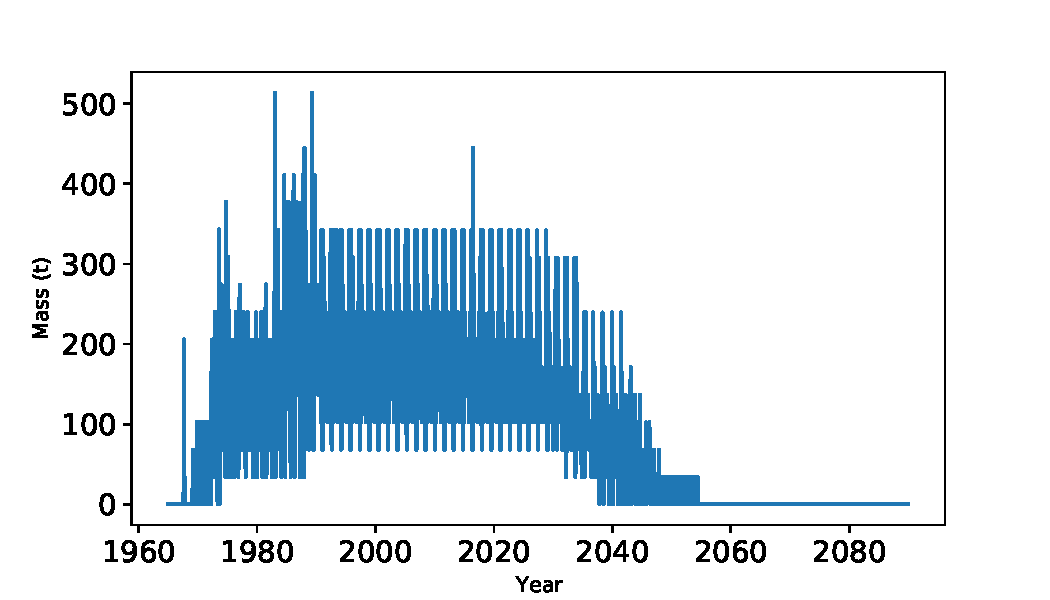
\includegraphics[scale=0.8]{s1_fuelsupply.pdf}
    \caption{Mass of uranium supplied to the LWRs in Scenario 1 at each time step.}
    \label{fig:fuel1}
\end{figure}

\begin{figure}
    \centering
    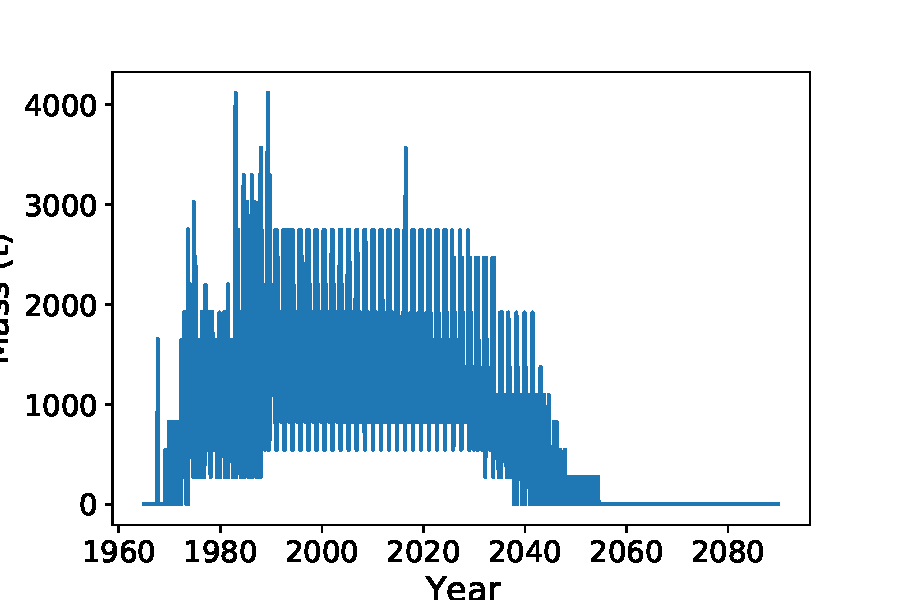
\includegraphics[scale=0.8]{s1_feed.pdf}
    \caption{Mass of natural uranium required to supply the fuel sent to LWRs at each time step in Scenario 1.}
    \label{fig:feed1}
\end{figure}

\begin{figure}
    \centering
    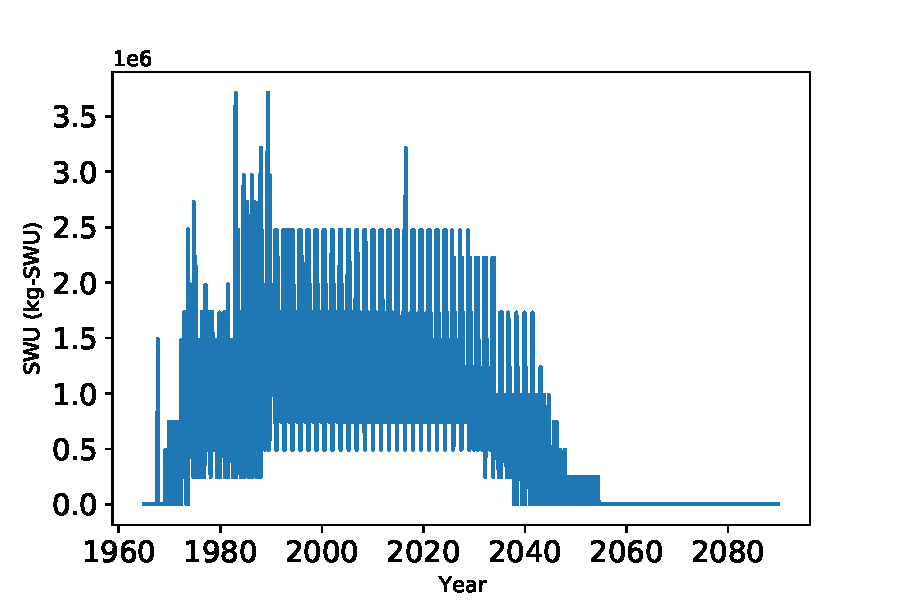
\includegraphics[scale=0.8]{s1_swu.pdf}
    \caption{SWU capacity required to enrich the uranium sent to LWRs at each time step in Scenario 1.}
    \label{fig:swu1}
\end{figure}

\section{Reactor deployment}

\section{Uranium resources}

\section{SWU capacity}

\section{Waste}